\documentclass[12pt, a4paper]{article}

% ===== 中文支持 =====
\usepackage[UTF8, zihao=-4]{ctex}

% ===== 页边距 =====
\usepackage[top=2.5cm, bottom=2.5cm, left=2.8cm, right=2.8cm]{geometry}

% ===== 字体 =====
\usepackage{fontspec}
\setmainfont{Times New Roman}

% ===== 行距 =====
\usepackage{setspace}
\setstretch{1.5}
\setlength{\parskip}{0pt}

% ===== 插图 =====
\usepackage{graphicx}
\usepackage{float}
\graphicspath{{./}}

% ===== 表格 =====
\usepackage{booktabs}
\usepackage{array}

% ===== 数学公式 =====
\usepackage{amsmath, amssymb}

% ===== 图表编号 =====
\usepackage{chngcntr}
\renewcommand{\thefigure}{\arabic{section}-\arabic{figure}}
\renewcommand{\thetable}{\arabic{section}-\arabic{table}}
\counterwithin{figure}{section}
\counterwithin{table}{section}

% ===== 图表标题格式 =====
\usepackage{caption}
\captionsetup{font=small, labelsep=space, justification=centering,
              aboveskip=6pt, belowskip=12pt}
\captionsetup[table]{aboveskip=12pt, belowskip=6pt, position=above}

% ===== 页眉页脚 =====
\usepackage{fancyhdr}
\setlength{\headheight}{15pt}
\pagestyle{fancy}
\fancyhf{}
\fancyhead[C]{\small 实验报告}
\fancyfoot[C]{\small\thepage}

% ===== 目录超链接 =====
\usepackage[colorlinks=true, linkcolor=black, citecolor=black, urlcolor=blue,
            bookmarks=true, bookmarksnumbered=true]{hyperref}

% ===== 章节标题格式 =====
\usepackage{titlesec}
\titleformat{\section}[block]
  {\centering\heiti\zihao{4}}{\thesection}{1em}{}
\titlespacing*{\section}{0pt}{24pt}{18pt}
\titleformat{\subsection}[hang]
  {\heiti\zihao{-4}}{\thesubsection}{1em}{}
\titlespacing*{\subsection}{0pt}{18pt}{6pt}
\titleformat{\subsubsection}[hang]
  {\heiti\zihao{-4}}{\thesubsubsection}{1em}{}
\titlespacing*{\subsubsection}{0pt}{12pt}{6pt}

\begin{document}

% ===== 封面 =====
\begin{titlepage}
  \centering
  \vspace*{3cm}
  {\heiti\zihao{2} 实验报告} \\[1cm]
  {\heiti\zihao{3} 马赫-曾德干涉实验} \\[2cm]
  \begin{tabular}{ll}
    姓\quad 名： & 叶哲昊 \\[0.5cm]
    学\quad 号： & 24012561 \\[0.5cm]
    实验日期：   & 2026年6月5日 \\
  \end{tabular}
  \vfill
\end{titlepage}

\tableofcontents
\newpage
\setcounter{page}{1}

\section{实验目的}

\begin{enumerate}
  \item 搭建并调节马赫-曾德干涉仪（Mach-Zehnder Interferometer，MZI），
        掌握精密光学系统的对准与调节方法。
  \item 观察平行双光束的干涉现象，理解分振幅干涉的基本原理。
  \item 通过改变两束光的夹角方向与大小，依次观察水平、竖直、粗细各异的等厚
        干涉条纹，以及近似平行时出现的类牛顿环同心圆弧条纹。
  \item 定性评估光学平台的隔振稳定性，观察外界振动对干涉条纹的影响。
\end{enumerate}

\section{实验原理}

\subsection{马赫-曾德干涉仪的光路结构}

马赫-曾德干涉仪是利用分振幅法产生双光束干涉的典型仪器。
如图~\ref{fig:schematic} 所示，整套光路由两块分光光楔（半反半透镜，
记为 BS1、BS2）和两块全反射镜（M1、M2）组成，
四个反射面互相接近平行，中心光路构成一个平行四边形。

\begin{figure}[H]
  \centering
  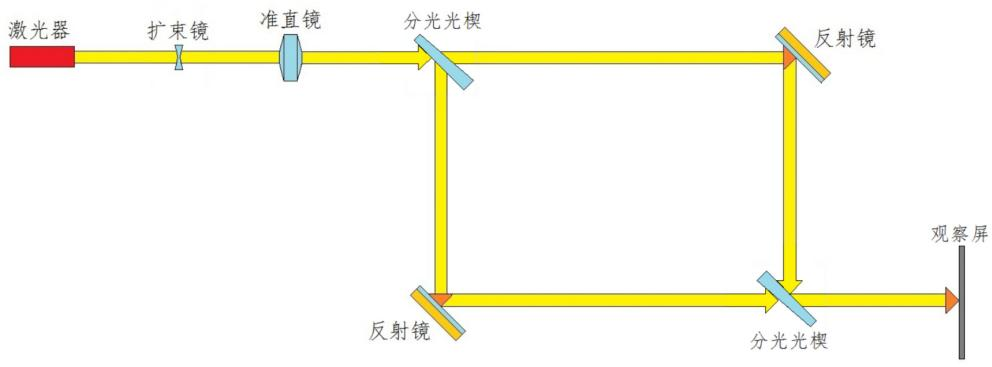
\includegraphics[width=0.85\textwidth]{images/66d819561c411d4e17076e3a0b957144799926455c07d222c4175ee6db8eaeb1.jpg}
  \caption{马赫-曾德干涉仪光路示意图}
  \label{fig:schematic}
\end{figure}

激光器出射的光束经空间滤波器（Spatial Filter）扩束滤波后，
再经准直镜（Collimating Lens，焦距 $f = 100\,\text{mm}$）
整形为宽度适当的平行光束，射入 BS1 后分为两路：
\begin{itemize}
  \item \textbf{光路 1（反射路）}：被 BS1 反射 $\to$ M1 全反射
        $\to$ 被 BS2 反射后输出；
  \item \textbf{光路 2（透射路）}：透过 BS1 $\to$ M2 全反射
        $\to$ 透过 BS2 后输出。
\end{itemize}
两路光在 BS2 后方的观察区域相遇，形成双光束干涉。

\subsection{干涉条纹的形成与间距}

设两束出射光在观察平面内的夹角为 $\theta$（小角近似），
激光波长为 $\lambda$。在观察平面上，光程差随横向位置 $x$ 线性变化：
\begin{equation}
  \delta(x) = x\sin\theta \approx x\theta
\end{equation}
相邻亮纹（相长干涉）之间的间距为：
\begin{equation}
  \Delta x = \frac{\lambda}{\theta}
  \label{eq:fringe_spacing}
\end{equation}
由式~\eqref{eq:fringe_spacing} 可知：夹角 $\theta$ 越大，条纹越密；
夹角趋于零时，条纹间距趋于无穷大，视场均匀无条纹。
若两束光在水平方向有夹角，则观察到竖直条纹；
若在竖直方向有夹角，则观察到水平条纹。

\subsection{类牛顿环条纹的成因}

当调节合束分光光楔使两束光接近平行（$\theta \to 0$），
但两束光存在微小的波面曲率差时（例如准直不完全导致的轻微球面波成分），
两束光的等相位面在空间中形成同轴旋转曲面，
干涉图样呈现以视场中心为圆心的同心圆弧，即类牛顿环条纹。

\section{实验仪器}

\begin{itemize}
  \item 绿色固体激光器（波长约 532\,nm）
  \item 可调衰减器
  \item 空间滤波器（显微物镜 + 针孔，针孔直径约 25\,$\mu$m）
  \item 准直镜（焦距 $f = 100\,\text{mm}$）
  \item 分光光楔（半反半透镜）$\times 2$
  \item 全反射镜 $\times 2$
  \item CMOS 工业相机（大恒光电 HV1351UM，分辨率 $1280 \times 1024$）
  \item 光学平台（大恒光电）及各类精密调节支架
\end{itemize}

\section{实验步骤}

\begin{enumerate}
  \item \textbf{调节激光器水平。}借助可变光阑（开孔约 2\,mm），
        分别在激光器近处和远处检查光斑位置，
        反复调节光阑高低与激光夹持器的水平俯仰旋钮，
        直至出射激光束与光学平台台面平行。调好后将可调衰减器安装到光路中。

  \item \textbf{调整空间滤波器。}将物镜安装于空间滤波器基座，
        调节三维位移台使扩束光斑打在光阑中心；
        安装 25\,$\mu$m 针孔，继续微调使聚焦光斑与针孔重合
        （以圆孔衍射环消失为准）。

  \item \textbf{调整准直镜。}将准直镜置于距空间滤波器针孔约 100\,mm 处，
        调节高度使出射光束通过光阑中心；
        前后移动准直镜，使近处与远处光斑大小一致，获得良好平行光束。

  \item \textbf{搭建马赫-曾德光路。}按平行四边形拓扑依次放置 BS1、M1、M2、BS2，
        使四个反射面接近互相平行；
        量取两路光光程，调节反射镜位置使两路光程大致相等；
        用光阑逐一检查各反射光束高度，确保均与台面平行。

  \item \textbf{调节两光斑重合。}微调一块全反射镜，
        使两束光在合束分光光楔出射面上重合；
        再微调合束分光光楔，使两束光在 CMOS 相机靶面上完全重合。

  \item \textbf{观测各类干涉条纹。}将 CMOS 相机与计算机连接，
        分辨率设为 $1280 \times 1024$，开启实时显示；
        微调合束分光光楔的倾斜角度，
        依次调出竖直粗条纹、竖直细条纹、水平粗条纹、水平细条纹
        及类牛顿环条纹，拍照记录各干涉现象。

  \item \textbf{光学平台稳定性观测。}在某一条纹状态下，
        轻拍光学平台或在台旁地面跳动，
        观察并记录干涉条纹受扰后的变化及恢复情况，
        定性评价光学平台的隔振能力。
\end{enumerate}

\section{实验现象记录}

本次实验共记录六类现象，包括实验装置全貌和五种干涉条纹图样，
全部通过实验照片记录如下。

\subsection{实验装置}

图~\ref{fig:setup} 为实验装置全貌照片，
可见光学平台上自左至右依次排布激光器、空间滤波器、准直镜、
两块分光光楔（BS1、BS2）、两块全反射镜（M1、M2）
以及 CMOS 相机和显示屏。

\begin{figure}[H]
  \centering
  
\includegraphics[width=0.85\textwidth]{实验照片/实验装置全貌.jpg}
  \caption{马赫-曾德干涉仪实验装置全貌}
  \label{fig:setup}
\end{figure}

\subsection{竖直干涉条纹}

图~\ref{fig:v_coarse} 和图~\ref{fig:v_fine} 分别为竖直粗条纹和竖直细条纹。
此时两束光在水平方向存在夹角 $\theta_h$，
干涉条纹呈竖直方向排列；增大 $\theta_h$，条纹间距 $\Delta x = \lambda/\theta_h$ 减小，
条纹变密（由粗变细）。

\begin{figure}[H]
  \centering
  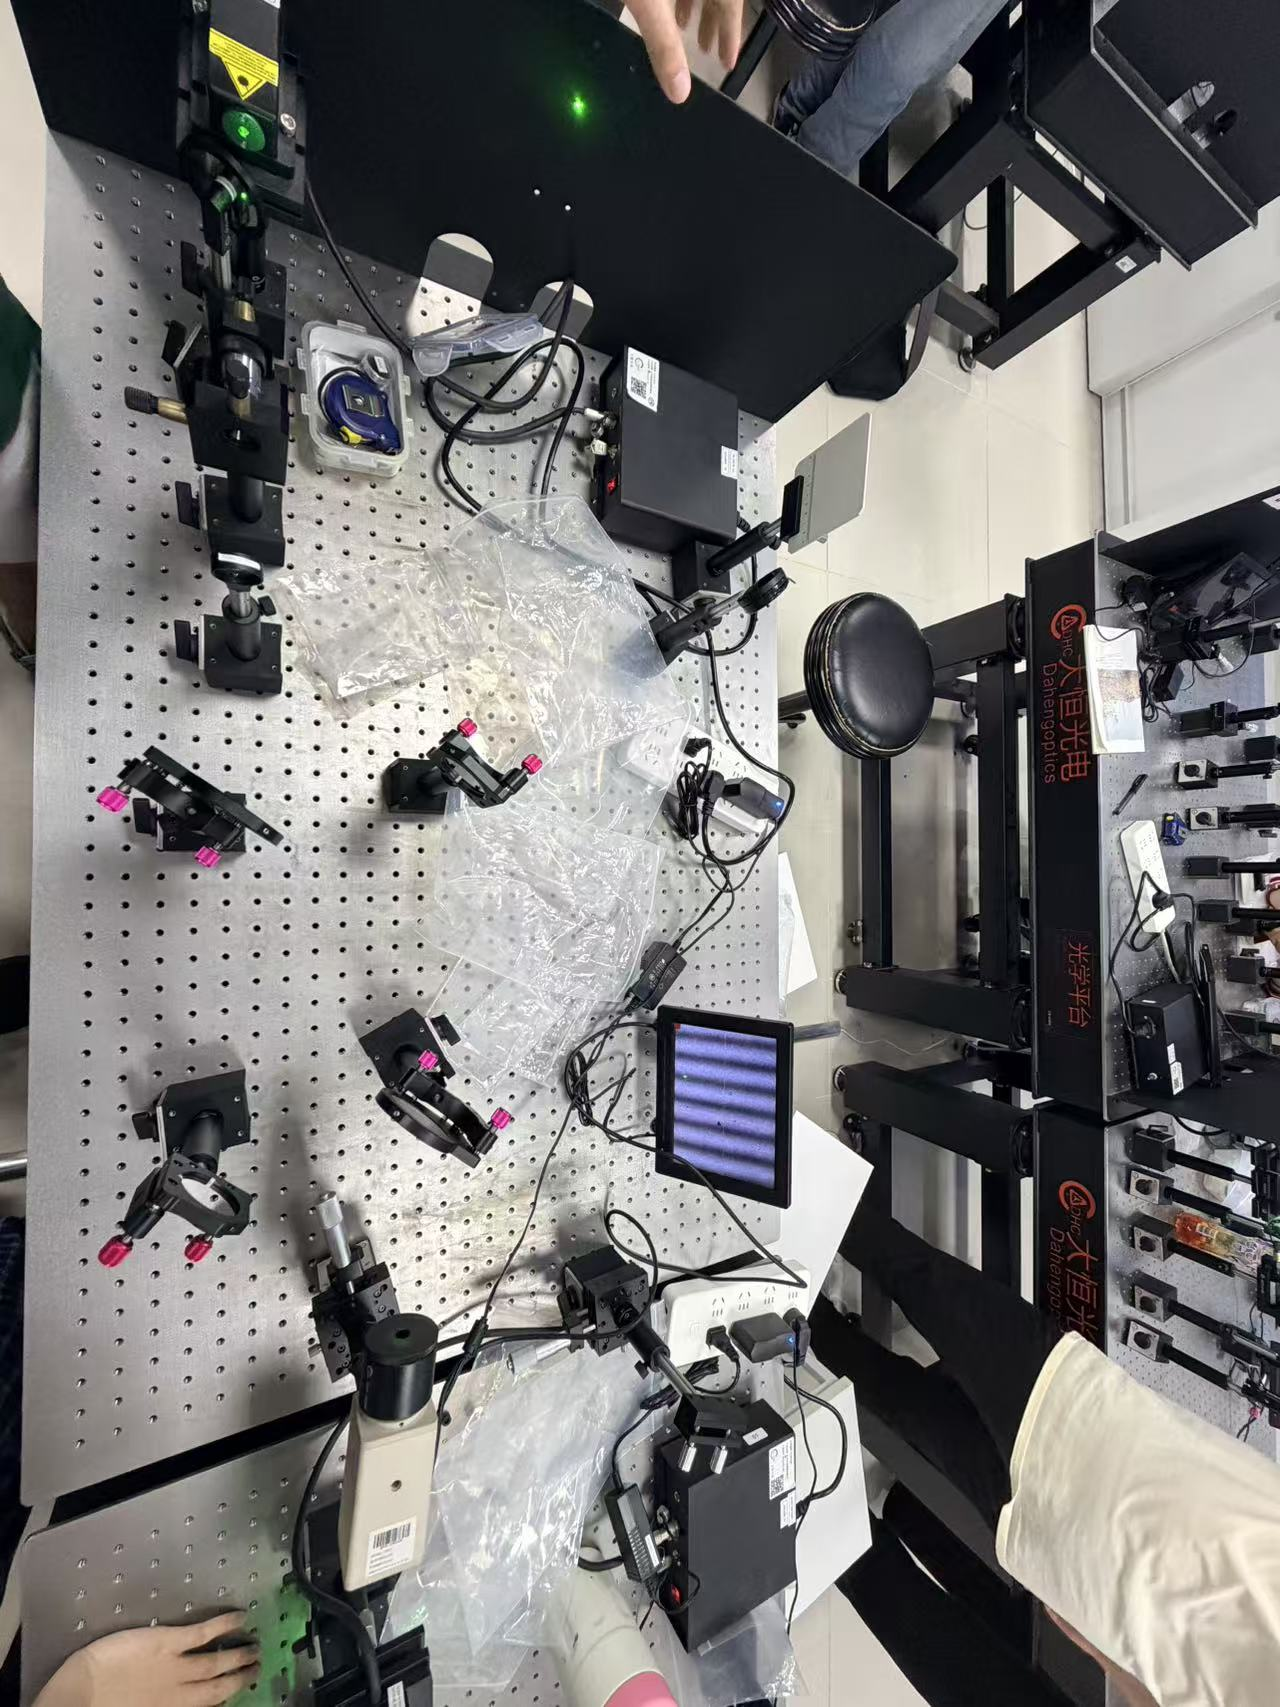
\includegraphics[width=0.72\textwidth]{实验照片/竖直粗条纹.jpg}
  \caption{竖直粗条纹（两束光水平夹角较小）}
  \label{fig:v_coarse}
\end{figure}

\begin{figure}[H]
  \centering
  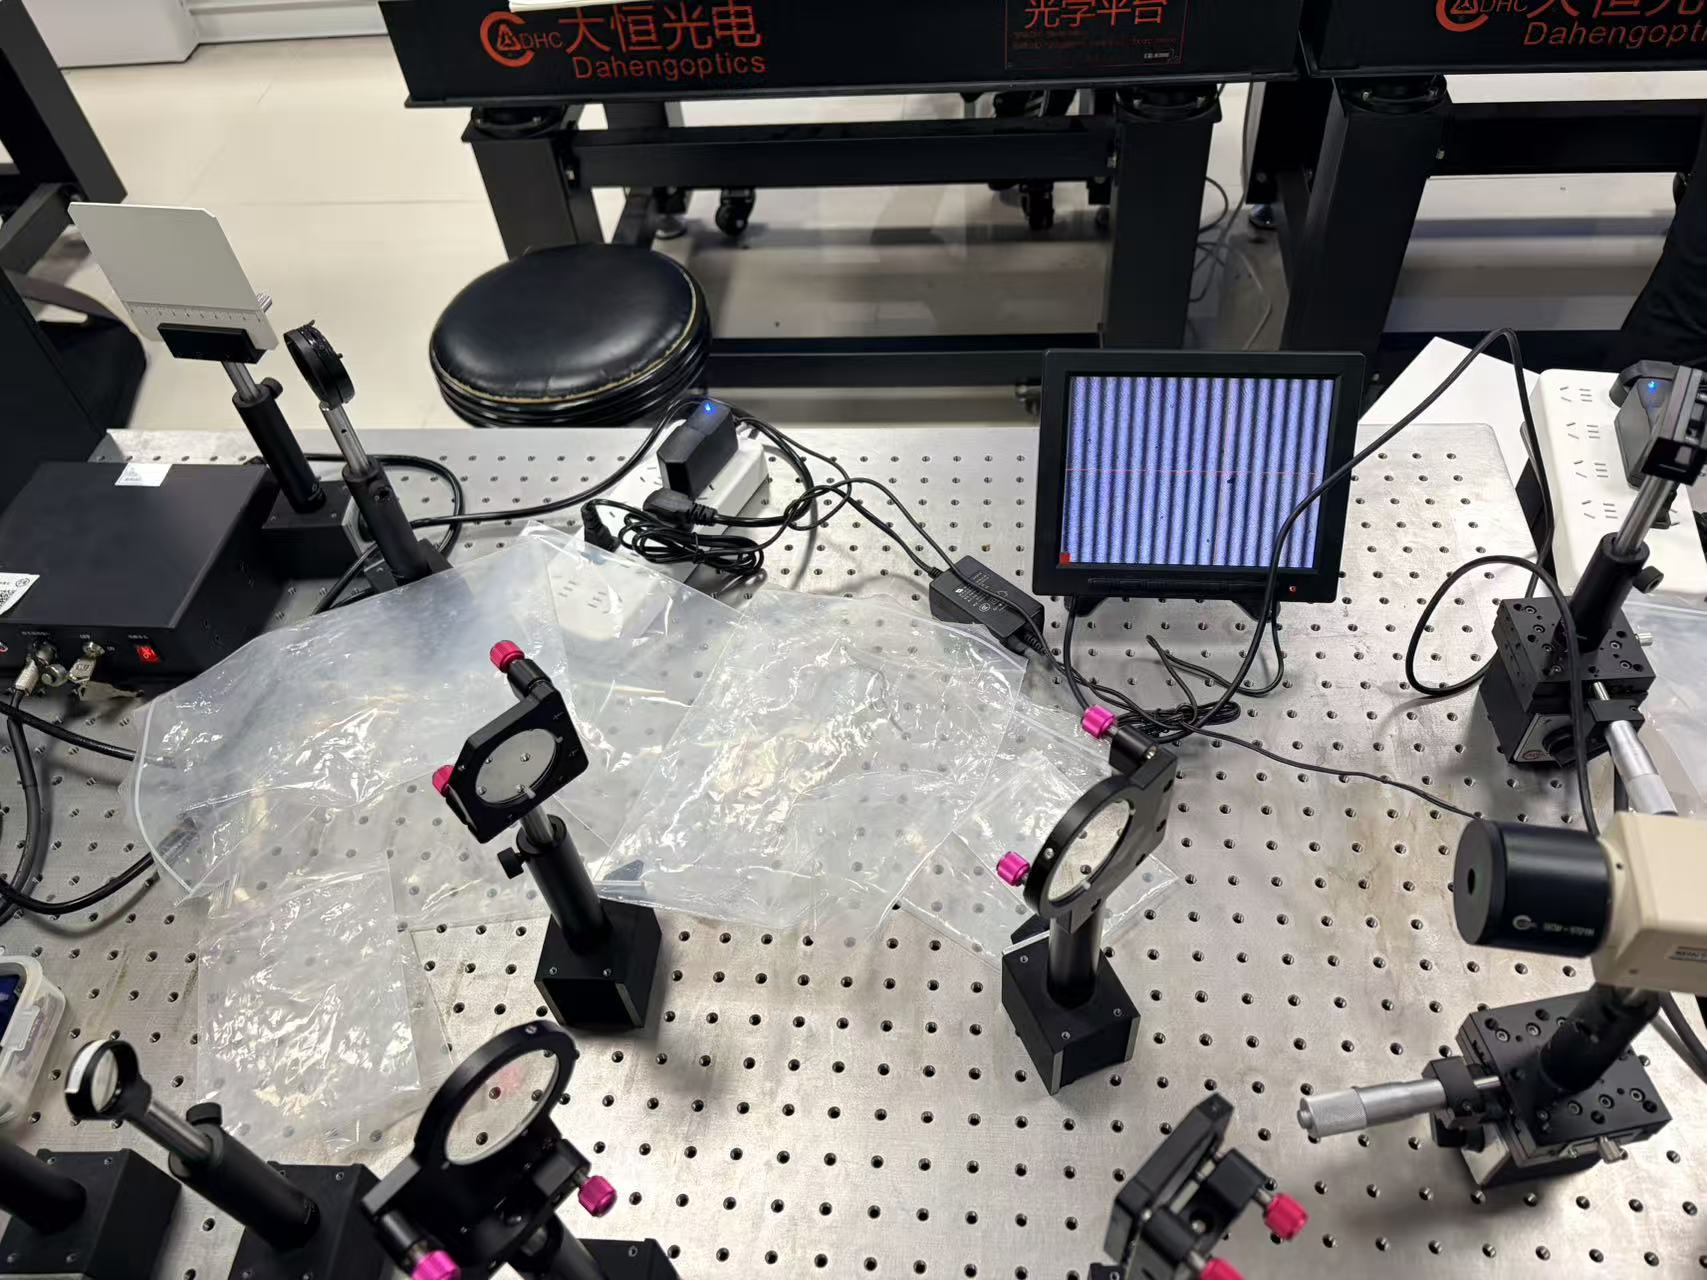
\includegraphics[width=0.72\textwidth]{实验照片/竖直细条纹.jpg}
  \caption{竖直细条纹（两束光水平夹角较大）}
  \label{fig:v_fine}
\end{figure}

\subsection{水平干涉条纹}

图~\ref{fig:h_coarse} 和图~\ref{fig:h_fine} 分别为水平粗条纹和水平细条纹。
此时两束光在竖直方向存在夹角 $\theta_v$，
干涉条纹呈水平方向排列；增大 $\theta_v$，条纹由疏变密。

\begin{figure}[H]
  \centering
  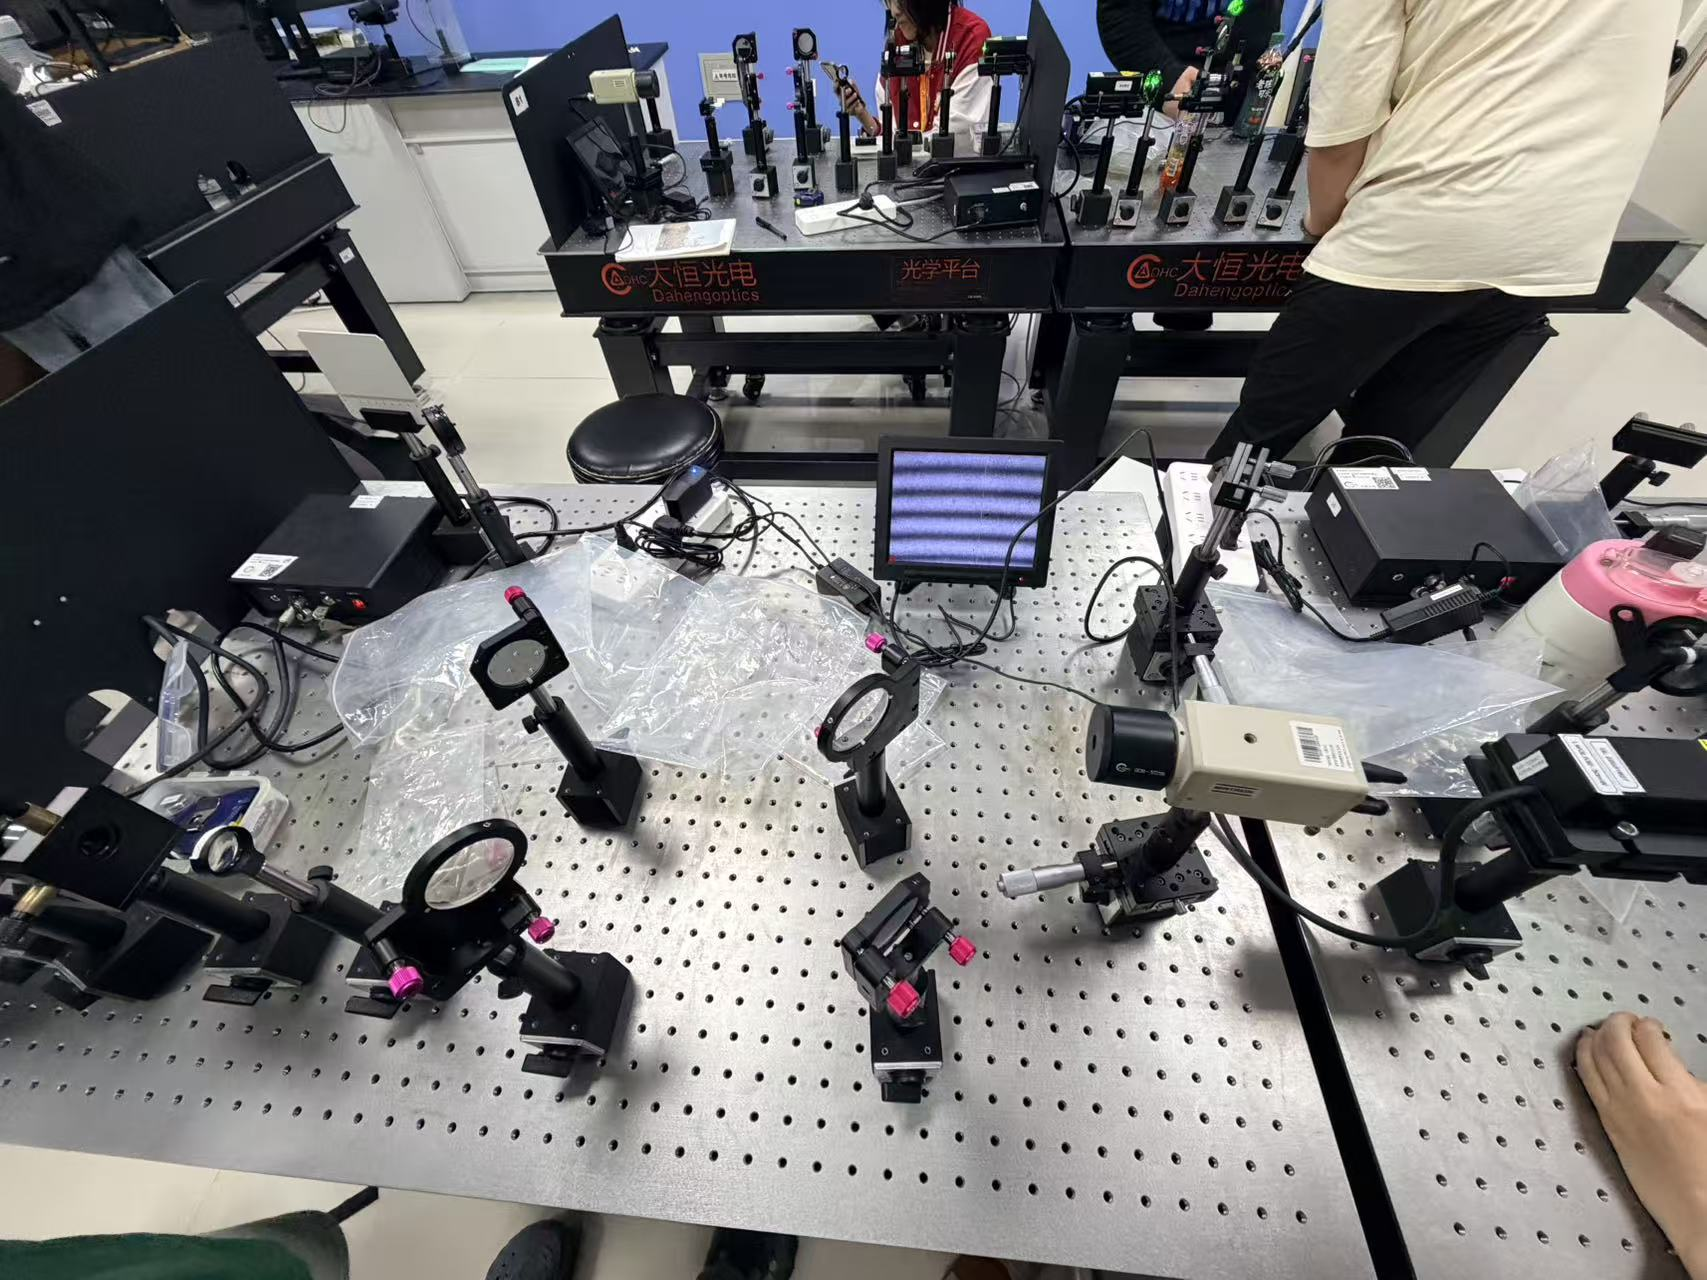
\includegraphics[width=0.72\textwidth]{实验照片/水平粗条纹.jpg}
  \caption{水平粗条纹（两束光竖直夹角较小）}
  \label{fig:h_coarse}
\end{figure}

\begin{figure}[H]
  \centering
  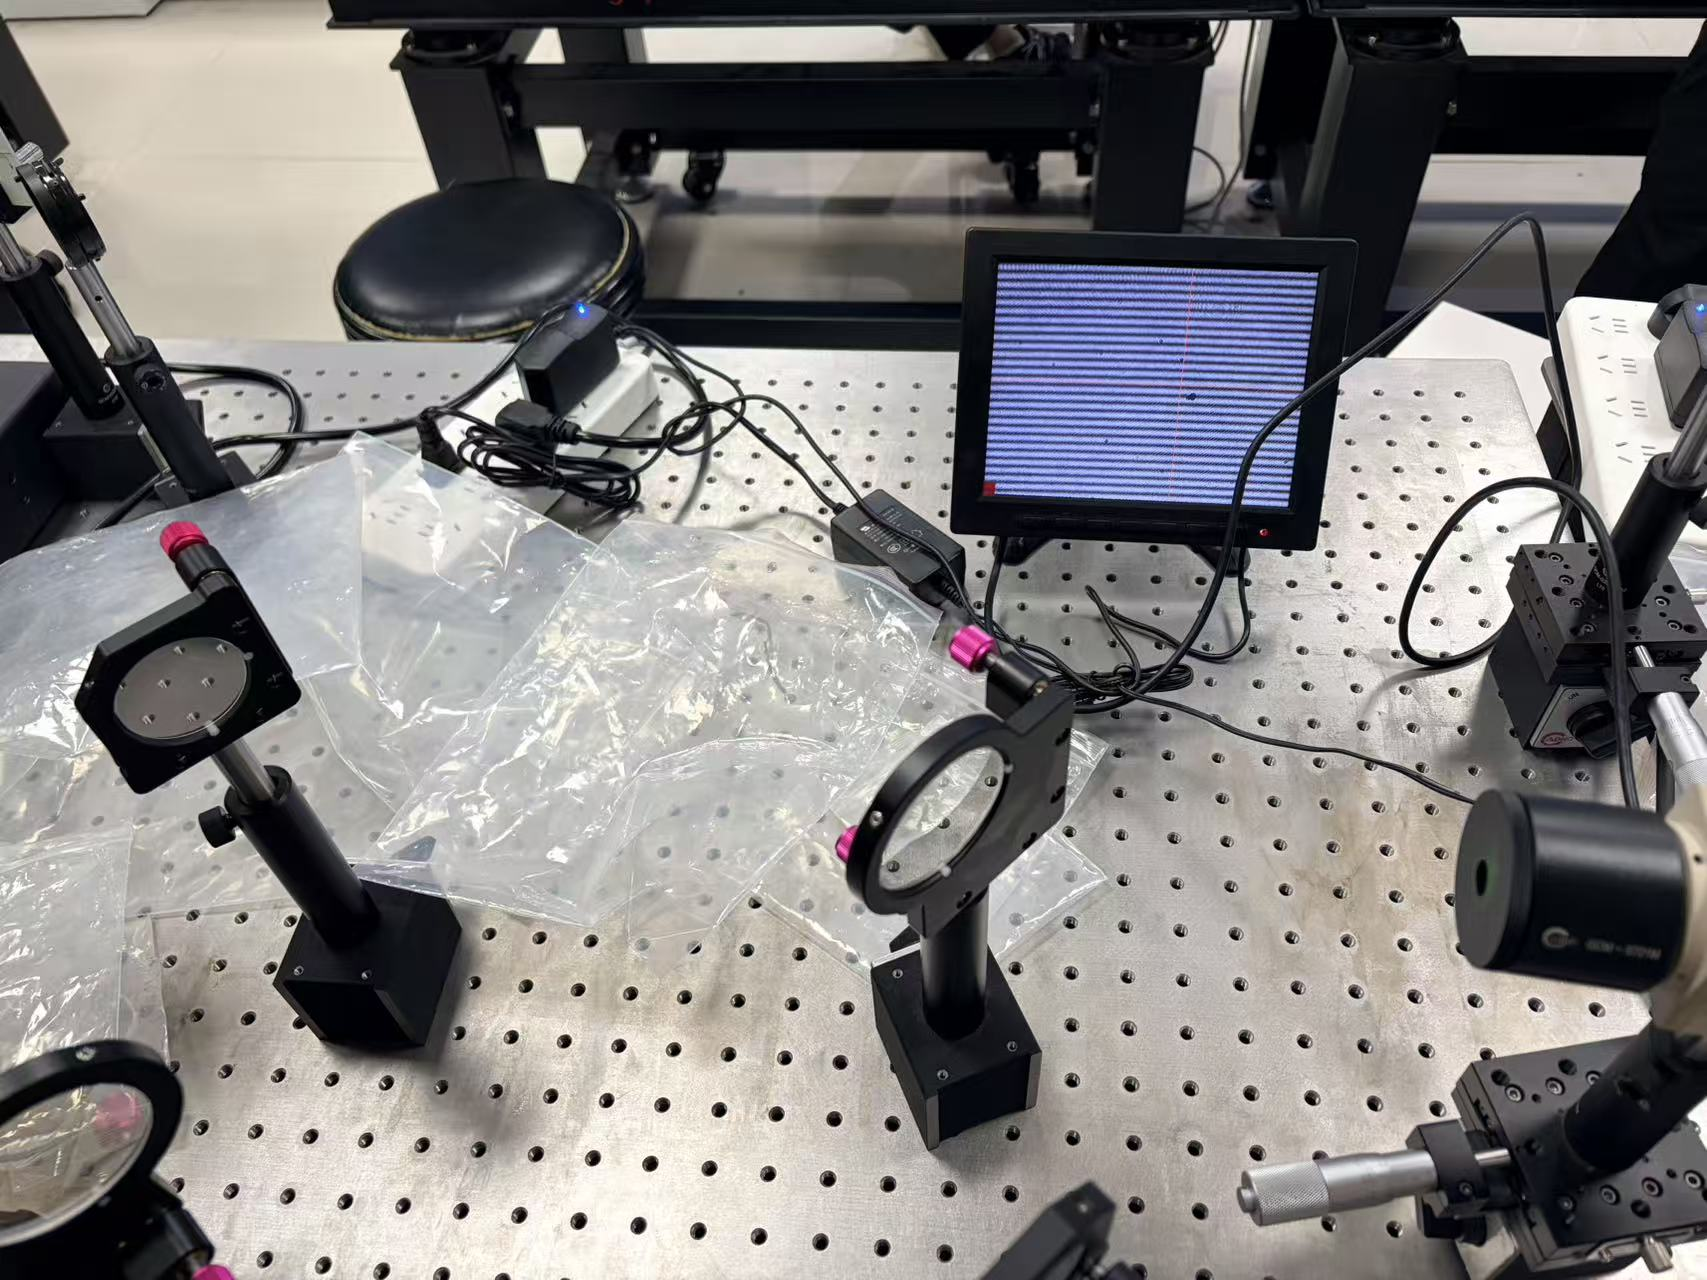
\includegraphics[width=0.72\textwidth]{实验照片/水平细条纹.jpg}
  \caption{水平细条纹（两束光竖直夹角较大）}
  \label{fig:h_fine}
\end{figure}

\subsection{类牛顿环条纹}

图~\ref{fig:rings} 为在白色观察屏上拍摄的类牛顿环干涉条纹。
当两束光近似平行时，波面曲率的微小不匹配使干涉条纹呈
以光斑中心附近为圆心的同心圆弧形，与牛顿环相似。

\begin{figure}[H]
  \centering
  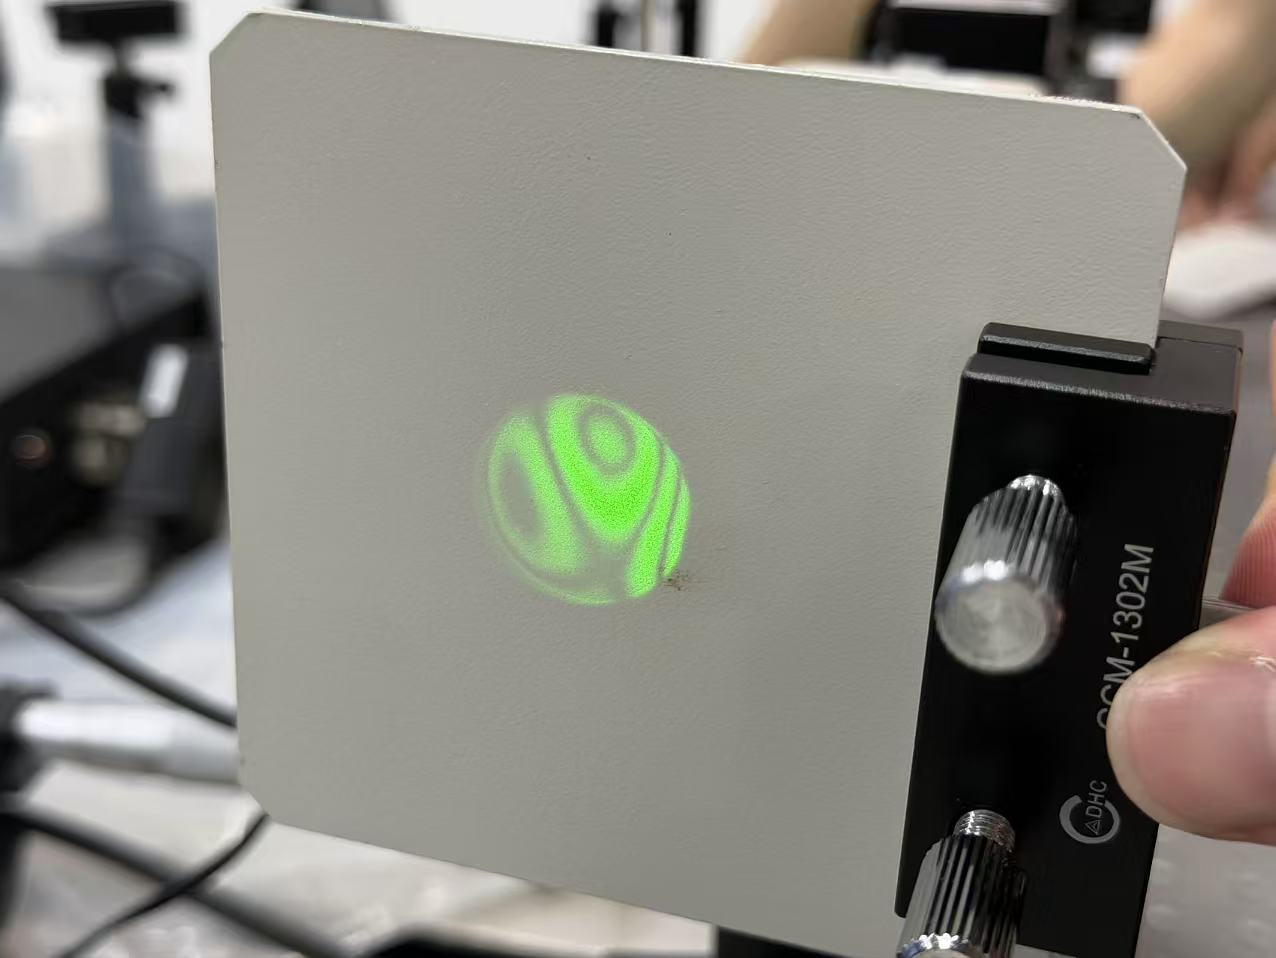
\includegraphics[width=0.55\textwidth]{实验照片/牛顿环条纹.jpg}
  \caption{类牛顿环干涉条纹（两束光近似平行时，在白色观察屏上记录）}
  \label{fig:rings}
\end{figure}

\section{实验结果与分析}

\subsection{条纹方向与夹角方向的对应关系}

实验观察表明，干涉条纹的走向与两束光夹角的方向互相垂直：
调节合束分光光楔使两束光产生水平夹角时，出现竖直条纹；
调节产生竖直夹角时，出现水平条纹。
这与理论分析一致——夹角方向决定光程差的空间梯度方向，
等光程差线（即亮纹）垂直于该梯度方向排列。

\subsection{条纹密度与夹角大小的关系}

由式~\eqref{eq:fringe_spacing}（$\Delta x = \lambda/\theta$）可知，
条纹间距与两束光夹角成反比。
实验中逐渐增大合束分光光楔的倾斜量，
观察到条纹从粗变细（间距从大变小），与理论预测定性吻合。

\subsection{类牛顿环条纹的分析}

在两束光趋近平行的过程中，条纹间距不断增大直至接近均匀照明。
调节至两束光波面存在微小球面曲率差时，出现图~\ref{fig:rings}
所示的类牛顿环同心圆弧条纹。
这是因为两束准平行光的等相差面在空间中形成旋转曲面，
截面为圆形，导致干涉图样呈环形分布。

\subsection{光学平台的稳定性}

轻拍光学平台后，CMOS 相机画面中的干涉条纹出现明显的位移和模糊，
随后在约数秒内逐渐恢复到稳定状态，表明大恒光电光学平台具有较好的被动隔振能力。
这验证了气浮/弹性隔振光学平台可有效衰减来自地面的低频振动。

\section{误差分析}

\begin{enumerate}
  \item \textbf{准直误差。}准直镜调节不完全时，出射光束存在微小发散角，
        导致两路光的波面曲率不完全匹配，影响条纹的均匀性与对比度。
  \item \textbf{等光程调节误差。}两路光光程的轻微差异
        （超过激光器相干长度时条纹对比度下降）
        会降低干涉条纹的可见度。
  \item \textbf{光学元件质量与安装偏差。}分光光楔和反射镜的表面疵病、
        平行度偏差等会引入额外的波像差，使条纹产生弯曲或不均匀。
  \item \textbf{振动与气流扰动。}实验室内的地面振动、声音振动以及空气热扰动
        是干涉条纹稳定性最主要的误差来源，
        会导致条纹随机漂移甚至短暂消失。
  \item \textbf{相机曝光与量化误差。}CMOS 相机的曝光时间设置不当
        （过曝或欠曝）会导致条纹对比度在图像中降低，
        影响条纹细节的记录质量。
\end{enumerate}

\section{思考题}

\subsection*{思考题 1：两臂为什么要尽量保证长度相等}

马赫-曾德干涉仪采用分振幅法，两束光来自同一激光源，但它们在分束后分别经过信号臂和参考臂，最后再重新合束。若要在观察屏上得到稳定、清晰的干涉条纹，除两束光需要空间重合、偏振态接近外，还必须使两臂的光程差小于光源的相干长度。设两臂光程差为 $\Delta L$，光源相干长度为 $L_c$，只有当
\begin{equation}
  |\Delta L| \lesssim L_c
\end{equation}
时，两束光在合束处仍保持较稳定的相位关系，干涉项才能保留下来。

从光强表达式看，两束光叠加后的强度可写为
\begin{equation}
  I = I_1 + I_2 + 2\sqrt{I_1 I_2}\,|\gamma(\Delta L)|\cos\Delta\varphi ,
\end{equation}
其中 $|\gamma(\Delta L)|$ 表示与光程差有关的相干度。当两臂光程差远大于光源相干长度时，$|\gamma(\Delta L)| \to 0$，干涉项在时间平均后基本消失。因此屏幕上不再出现稳定的明暗条纹，只能看到两束光强度的普通叠加，表现为对比度很低甚至完全无条纹的光斑。

\subsection*{思考题 2：沿光轴移动观察屏时条纹间距是否改变}

在本实验调出的直条纹状态下，马赫-曾德干涉仪更接近于两束平面波之间形成的楔形空气层干涉，即等厚干涉，而不是平行平板的等倾干涉。两束出射光存在小夹角 $\theta$ 时，相位差随横向坐标 $x$ 改变：
\begin{equation}
  \Delta\varphi(x) = \frac{2\pi}{\lambda}x\sin\theta + \varphi_0 .
\end{equation}
相邻亮纹满足相位差相差 $2\pi$，所以条纹间距为
\begin{equation}
  \Delta x = \frac{\lambda}{\sin\theta} \approx \frac{\lambda}{\theta}.
\end{equation}
可见条纹间距主要由波长 $\lambda$ 和两束光夹角 $\theta$ 决定，而不是由观察屏到合束器的距离决定。

因此，在两束光仍能较好重合、夹角不变且波面近似为平面波的条件下，沿光轴前后移动观察屏时，直条纹的间距基本不变；可能改变的是条纹整体位置、光斑重合区域和清晰度。若屏幕移动较远，使两束光的重合面积变小，或实际光束存在明显发散和波面曲率差，则观察到的条纹对比度和局部形状可能发生变化，但这不属于理想等厚干涉条纹间距由传播距离决定的情形。

\subsection*{思考题 3：操作中如何实现等厚干涉与等倾干涉}

本实验中实现等厚干涉时，先使两束光在合束后空间重合，再有意微调合束分光光楔或某一反射镜的倾角，使两束出射光之间保留一个很小的夹角。此时两束波面相当于构成一个楔形空气层，光程差沿某一横向方向近似线性变化，于是观察到一组平行直条纹。判断依据是：条纹近似平直且互相平行；条纹方向与两束光夹角方向垂直；继续增大夹角时条纹变密，减小夹角时条纹变疏。

实现等倾干涉时，则需要把两束光调到尽量平行，使近处和远处的两光斑都尽量重合，尽量消除两束光之间的线性夹角。若此时两束光仍存在轻微的波面曲率差，或者等效为不同倾角的光束分量发生干涉，就会出现类似牛顿环的同心圆弧条纹。判断依据是：条纹不再表现为单一方向的平行直线，而是呈圆环或圆弧形分布；微调反射镜倾角时，圆环中心会移动，条纹可能向中心收缩或向外扩展；当两束光进一步偏离平行时，圆环条纹会逐渐过渡为直条纹。

\subsection*{思考题 4：MZI 型电光调制器的工作原理}

若在马赫-曾德干涉仪的一臂中插入电光晶体（如铌酸锂），并在晶体上施加电压，则该臂中光的折射率会因线性电光效应（Pockels 效应）而改变。设晶体长度为 $L$，折射率变化为 $\Delta n(V)$，则该臂引入的附加相位差为
\begin{equation}
  \Delta\varphi(V) = \frac{2\pi}{\lambda}\Delta n(V)L .
\end{equation}
由于 $\Delta n(V)$ 与外加电压近似成正比，外加电压就可以连续控制两臂之间的相位差。

两束光在输出端合束后，输出光强由相位差决定：
\begin{equation}
  I_{\mathrm{out}} = I_1 + I_2 + 2\sqrt{I_1 I_2}
  \cos\!\left[\Delta\varphi_0 + \Delta\varphi(V)\right] .
\end{equation}
当电压使两臂相位差满足相长干涉条件时，输出光强较大；当电压使相位差增加到相消干涉条件时，输出光强变小。通常用半波电压 $V_\pi$ 表征调制能力，即电压改变 $V_\pi$ 时两臂相位差改变 $\pi$，输出端可由亮态转为暗态，或由暗态转为亮态。因此，通过调节外加电压，可以把电信号转换为输出光强的变化，实现 MZI 型电光强度调制。

\section{实验结论}

本实验成功搭建并调通了马赫-曾德干涉仪，通过 CMOS 相机
和白色观察屏完整记录了多种干涉条纹现象，主要结论如下：

\begin{enumerate}
  \item 实验观察到竖直粗条纹、竖直细条纹、水平粗条纹、水平细条纹
        及类牛顿环五类干涉图样，各类条纹均清晰可辨，对比度良好。
  \item 条纹方向由两束光的夹角方向决定，条纹间距随夹角增大而减小，
        与理论公式 $\Delta x = \lambda/\theta$ 定性吻合。
  \item 两束光趋近平行时，干涉图样从平行条纹过渡为类牛顿环同心圆弧，
        证明微小波面曲率差对近平行双光束干涉图样有显著影响。
  \item 轻拍光学平台后，条纹在数秒内恢复稳定，
        定性验证了隔振光学平台良好的被动减振效果。
\end{enumerate}

\end{document}
